\begin{tikzpicture}[
font=\small,
>=stealth,
imgnode/.style={inner sep=0, outer sep=0},
label/.style={anchor=north}]
\newlength{\imgw}
\newlength{\imgh}

\setlength{\imgw}{0.25\textwidth}   % 3 Panels → 0.75\textwidth + gaps
\setlength{\imgh}{\dimexpr\imgw*510/825\relax}
\pgfmathsetmacro{\gap}{0.0833*\textwidth} 

  
% === Panel 1: ===
\node[imgnode] (img1) at (0,0) {
    \centering
    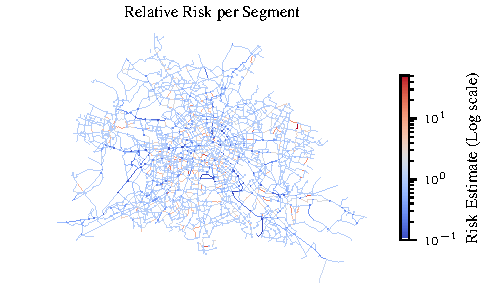
\includegraphics[width=\imgw,height=\imgh , trim=25pt 25pt 25pt 25pt, clip]{figs/risk_segments.pdf}
};
\node[label, below=3pt of img1] (label1) {\small(a) Risk levels Berlin area};

% === Panel 2: ===

\pgfmathsetmacro{\xtwo}{\imgw + \gap}
\node[imgnode] (img2) at (\xtwo pt, 0) {
    \centering
    \includegraphics[width=\imgw,height=\imgh , trim=29pt 52.2pt 29pt 32.2pt, clip]{figs/risk_map_final.pdf}
};
\node[label, below=3pt of img2] (label2) {(b) Junction 2482 with Accidents};

% === Panel 3:  ===
\pgfmathsetmacro{\xthree}{2*\imgw + 2*\gap}
\node[imgnode] (img3) at (\xthree pt, 0) {
    \centering
    \includegraphics[width=\imgw,height=\imgh , trim=20pt 0 20pt 0, clip]{figs/Streetview.jpeg}
};
\node[label, below=3pt of img3] (label3) {(c) Street View of Junction 2482};
\end{tikzpicture}